\documentclass[../main.tex]{subfiles}

\begin{document}
\section{Detecting and avoiding spectral pollution}

We now turn to methods of detecting or
avoiding spurious eigenvalues, which is a large focus of research in the area of
numerical spectral theory.

This section will mostly stick to heuristic derivations and numerical examples.
Proofs are often highly non-trivial, and tend to be worth an entire paper to
themselves (e.g. \cite{soussi2006convergence}) or are currently open problems
(e.g. \cite{chandler-wilde2012spectrum}).

\subsection{Second-order relative spectrum}
One method of detecting true eigenvalues (but not necessarily ruling out false ones,
as we will see) is the \emph{second-order relative spectrum} first defined by Levitin and Shargorodsky;

\begin{definition}{\textbf{(Second order relative spectrum \cite{levitin2002spectral})}}
  \index{second order relative spectrum}
  Let $A$ be a self-adjoint operator on a Hilbert space $\hilbert$, and 
  $\mathcal{L}$ a finite-dimensional subspace of $\hilbert$. Then the second-order relative
  spectrum of $A$ relative to $\mathcal{L}$ is defined as the set of all $z \in \mathbb{C}$
  such that $P_{\mathcal{L}}(A - z)\big|_{\mathcal{L}}$ is not invertible.
\end{definition}

This quantity is more difficult to calculate numerically than the regular Ritz matrix (owing to
it being a quadratic eigenvalue problem, rather than a linear one), but in some cases can allow
one to conclusively confirm that part of the spectrum does exist.

\begin{theorem}
  If $z$ is in the second-order relative spectrum of $A$ relative to some finite subspace $\mathbb{L}$,
  then
    $$\Spec(A) \cap [\mathrm{Re}(z) - |\mathrm{Im}(z)|, \mathrm{Re}(z) + |\mathrm{Im}z|] 
    \neq \emptyset.$$
\end{theorem}

That is, for any point $z$ in the second-order relative spectrum,
a circle centred on $\mathrm{Re}(z)$ with radius $|\mathrm{Im}(z)|$ is guaranteed to contain
a genuine part of the spectrum. Of course, as we are numerically approximating the second-order
spectrum there may be eigenvalues missing (indeed, is it possible for the second-order spectrum to
have pollution of its own?), so we cannot guarantee that a point outside of these circles is
definitely polluting; but it gives a strong piece of evidence towards where genuine eigenvalues
may be.

A standard way of solving quadratic eigenvalue problems is to convert them to linear ones. In
this case, the linearised problem is the generalised eigenvalue problem with block matrices
  $$
  \begin{pmatrix*}[c]
    PA^2 &  0 \\
    0    & -I
  \end{pmatrix*}
  \begin{pmatrix*}[c]
    u \\ v
  \end{pmatrix*}
  =
  \lambda
  \begin{pmatrix*}[c]
    2PA & I \\
    I   & 0
  \end{pmatrix*}
  \begin{pmatrix*}[c]
    u \\ v
  \end{pmatrix*}
  $$
where $(u, v)^T$ is a vector in $\mathcal{L} \times \mathcal{L}$. This is a simple enough method that
it is implemented in most computational linear algebra libraries, but has problems with numerical
stability and sensitivity \cite{higham2008scaling} - of course, how much this matters depends
heavily on $A$ (and on $A^2$, which may be significantly more complex!)

In Figure \ref{fig:sors-mult} one can see the second-order relative spectrum of the multiplication
operator on [0, 1] with symbol
$$f =
\begin{cases}
  x & x < 1/2 \\
  x + 1/2 & otherwise
\end{cases}.
$$
We have seen previously that the spectrum of this operator is $[0, 1/2] \cup [1, 3/2]$. In this case,
the second-order relative spectrum is affirmative of that, but it doesn't do much to rule out the
pollution we found between the gaps - there are parts of the second-order spectrum with large imaginary
part that stop us from ruling the entire gap out. However, if there \emph{were} an eigenvalue in the gap,
and a point of second-order spectrum with small imaginary part near it, that would allow us to conclude that
such an eigenvalue \emph{does} exist.

\begin{figure}[h!]
\centering
  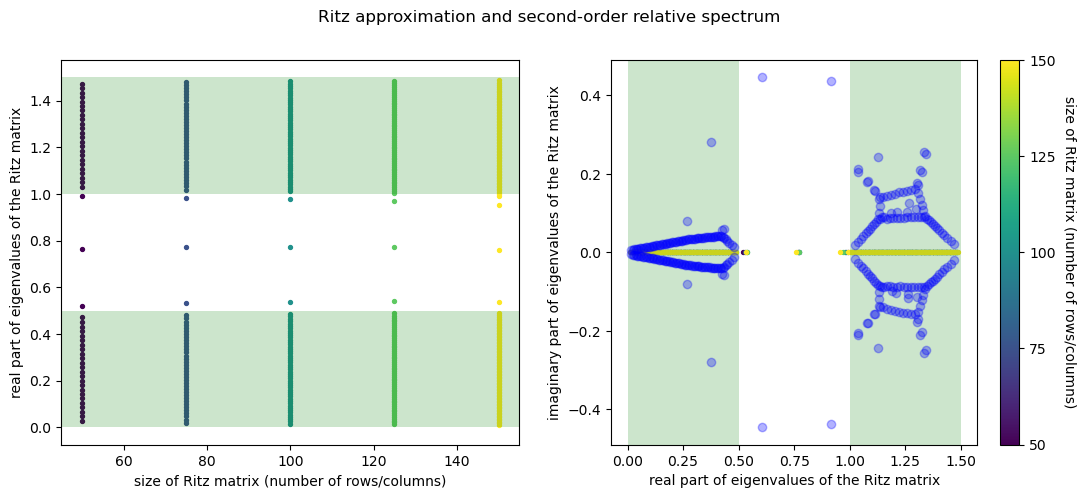
\includegraphics[width=0.9\linewidth, height=6cm]{sors}
  \caption{The spectrum of the multiplication operator with symbol described above, with the second-order
  relative spectrum overlaid in blue. Note the 'circle' of highly imaginary values that prevent us from
  ruling out pollution anywhere in the essential numerical range of the operator!}
  \label{fig:sors-mult}
\end{figure}

\subsection{Properties of eigenfunctions}
If there are only a small number of eigenvalues which we would like to learn
more about (e.g. once we have whittled down some of the pollution via a
dissipative barrier), it may be useful to then look at the eigenfunctions for
each relevant value. Polluting eigenvalues have rather interesting-looking
eigenfunctions (Figure \ref{fig:eigfuncs})

\begin{figure}[h!]
  \centering
  \begin{subfigure}{0.4\textwidth}
    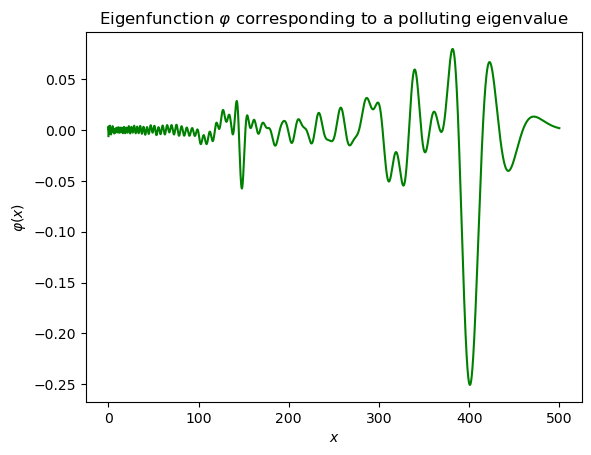
\includegraphics[width=0.9\linewidth, height=6cm]{poll-eig}
  \end{subfigure}
  \begin{subfigure}{0.4\textwidth}
    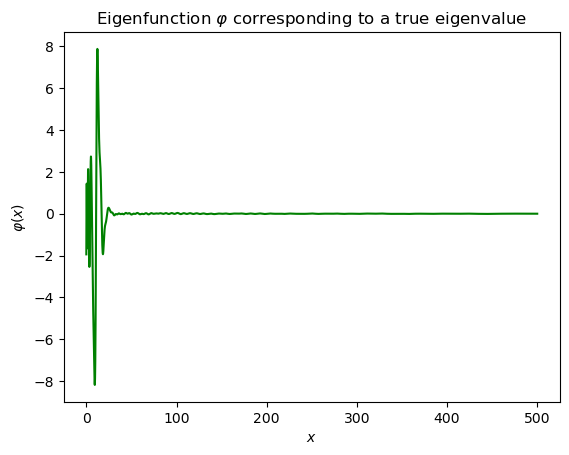
\includegraphics[width=0.9\linewidth, height=6cm]{real-eig}
  \end{subfigure}
  \caption{The eigenfunctions
  for a polluting and genuine eigenvalue of the operator in Example \ref{ex:aceto}
  below.}
\label{fig:eigfuncs}
\end{figure}

In some cases (below, we will prove this for a Sturm-Liouville operator on the
half-line), we can prove that there is a specific structure to the eigenfunctions -
for example, on $L^2[0, \infty)$, they must satisfy regularity and decay properties.

\begin{theorem}[adapted from\cite{aljawi2023eigenvalues}]
  Let $u$ be a solution of the boundary value problem 
    $$ 
    \begin{cases}
	-u'' + qu = \lambda u \\
	u(0) = 0
    \end{cases} 
    $$ 
  on $[0, \infty)$, and let $\mathrm{dist}(\lambda, \Spec_e(-\Delta + q)) > 0$.
  Then $u(x) = \exp(-\alpha x) v(x)$ for some function $v \in H_1^0 \cap H^2_{loc}$
  (i.e. $v$ is globally weakly differentiable once, locally weakly differentiable twice,
  and zero on the boundary) and 
  $\alpha^2 \in (0, c\cdot\mathrm{dist}(\lambda, \Spec_e(-\Delta + q)))$
  for $c \in (0, 1)$.
\end{theorem}
\begin{proof}\emph{(sketch)}
This is a modification of a theorem in \cite{aljawi2023eigenvalues} with an adjustment
to apply to eigenvalues of the problem. First we choose $b \geq 0$, and let $T_{b}$
be the Sturm-Liouville operator with Dirichlet boundary conditions on $[b, \infty)$.
Then if $b$ is such that $u(b) \neq 0$, we have $u \in \Dom(T_0)$ but not $\Dom(T_b)$.

Now let us choose a twice-differentiable function $w$ with compact support, such that
$w(b) = u(b)$, and let $\tilde{u(x)} = u(x) - w(x)$. Then $\tilde{u}$ is not an
eigenfunction of $T_b$:

  $$(T_b - \lambda)\tilde{u} 
    = (-\frac{d^2}{dx^2} + q - \lambda)(u - w)
    = (-\frac{d^2}{dx^2} + q - \lambda)w \neq 0$$

It can be shown that $\Spec_e(T_b)$ is the same for all $b$ \cite{akhiezer2013theory}.
  We can now invoke (a simplification of) Lemma 3.1 in \cite{aljawi2023eigenvalues}:
\begin{displayquote}
  Suppose $v$ solves the inhomogeneous boundary value problem
  $$
  \begin{cases}
    (-\frac{d^2/dx^2} + q - \lambda)v = (-\frac{d^2/dx^2} + q - \lambda)F
    v(0) = 0
  \end{cases}
  $$
  on $(b, \infty)$, and suppose there exists $\alpha$ such that
  $\mathrm{dist}(\lambda, \Spec((-\frac{d^2/dx^2} + q)) > \alpha > 0$.
  Then $v$ admits a representation $v(x) = e^{-\alpha(x-b)}\tilde{v}(x)$, where
  $\tilde{v}$ is weakly differentiable, twice-weakly differentiable locally,
  and zero on the boundary.
\end{displayquote}
We can then recover our original eigenfunction to be in the same form.
\end{proof}

\subsection{Dissipative barrier methods}
\label{sec:dissipative-barrier}
\index{dissipative barrier method}
Perhaps one of the most elegant methods for separating eigenvalues from spectral
pollution, albeit one with a wide variety of interesting behaviour,
is the dissipative barrier method. This method leverages finite-rank
perturbation of an operator.

Take an operator $T$ on a Hilbert space, and let $P$ be an orthonormal
projection onto a finite-dimensional space  such that for an eigenvector $u$,
$\|Pu - u\|$ is sufficiently small. Let $\lambda$ be the eigenvalue for $u$.
Then for the operator $T+iP$,
$$(T+iP) u = Tu + iPu \approx \lambda u + iu = (\lambda + i)u.$$
i.e. $(\lambda + i)$ is approximately an eigenvalue for $T+iP$. 

Then, the eigenvalues of the perturbed operator will have imaginary part of
approximately 1, and the set of eigenvalues produced by the approximation can be
filtered to discard points without imaginary part close to 1 as being pollution.
This is particularly useful for self-adjoint operators, where the entire
spectrum and the essential numerical range are a subset of the real line; in
that case, the perturbed eigenvalues will be the only points on the spectrum
with significant imaginary part. Even better, if the operator is also bounded,
then all pollution is in the essential numerical range (Theorem \ref{thm:pokrzywa}) which is
invariant under compact perturbation (Theorem \ref{thm:ess-ran-compact-ptb}) so the pollution will
converge to the real axis.

Let us see this concretely with an example.

\begin{example} 
  We return once again to our discontinuous multiplication
  operator $M_f$ on $L^2(0, 1)$ with symbol 
    $$
    f: x \mapsto 
    \begin{cases}
      x & x < 1/2\\
      x+1/2 & \text{otherwise}.
    \end{cases} 
    $$
  This time, we add a `rank-one perturbation' to get the operator 
  $\tilde{M}$ which has the action 
    $$\tilde{M}u = M_fu + (u, \varphi) \varphi,$$
  where $\varphi$ is a real-valued function on $L^2(0, 1)$.
  Then $\tilde{M}$ has an eigenvector: we rearrange to get
  \begin{align*} 
    f(x)u(x) + (u, \varphi)\varphi(x) & = \lambda u(x),\\
    \text{therefore }(\lambda - f(x))u(x) & = (u, \varphi)\varphi(x),\\
    u(x) & = c \frac{\varphi(x)}{\lambda - f(x)}
  \end{align*} 
  for some constant $c$. We then normalise this to
  $\frac{\varphi(x)}{\lambda - f(x)}$, which requires 
  \begin{align*}
    f(x)u + (u, \varphi)\varphi & = \lambda u \\
    (f(x) - \lambda)c\frac{\varphi(x)}{\lambda - f(x)} +
    (\frac{c\varphi}{\lambda - f}, \varphi)\varphi(x) & = 0 \\ -1 +
    (\frac{\varphi}{\lambda - f}, \varphi) & = 0 
  \end{align*}
  so we can normalise provided that
  $(\frac{\varphi}{\lambda - f}, \varphi) 
  = \int_0^1 \frac{|\varphi|^2}{\lambda - m} = 1.$
\end{example}

Thus for any value $\lambda$ we can choose $\varphi \in L^2(0, 1)$ and scale it
so that $\int_0^1 \frac{|\varphi|^2}{\lambda - m} = 1$ to get an operator
$\tilde{M}$ with spectrum $\Spec(M) \cup \{\lambda \in \mathbb{C} : \int_0^1
\frac{|\varphi|^2}{\lambda - m} = 1\}$. In Figure \ref{fig:nodbm} we can see the
results of Ritz approximations with $\varphi$ chosen such that the operator has
an eigenvalue at 0.7.\footnote{In particular, $\varphi$ was chosen to be the
constant $(\log(3) - 3\log(2) + \log(5) + \log(7) - \log(10))^{-1}$; this
satisfies the normalisation condition at $\lambda = 0.7$ but also at $\lambda
\approx 4.4$; the eigenvalue at $\lambda \approx 4.4$ has been cropped out of
the figure to improve illustration of the idea.} In Figure \ref{fig:dbm} we see
the same approximation but with the dissipative barrier $iP$ where $P$ is the
projection onto $\mathrm{span}\{\phi_n, |n| \leq 25\}$. Note that the spectrum
on the line ${(x, y) : \mathrm{Imag}(x) = 1}$ converges to what we'd expect the
spectrum to be.

\begin{figure}[p!] 
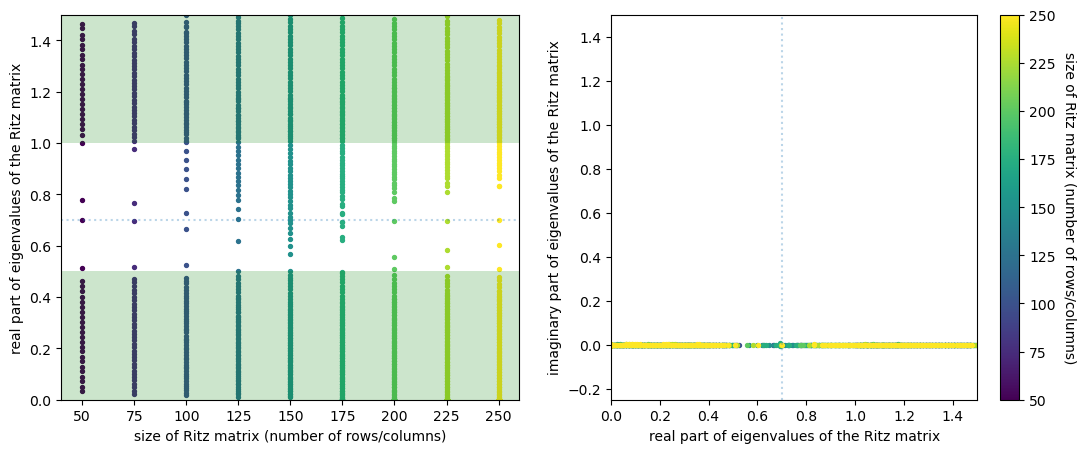
\includegraphics[width=0.9\linewidth, height=6cm]{ptb-mult-nodbm}
\caption{The real part of the approximate spectrum for $\tilde{M}$; on the
	left, the real parts of the approximate
	spectrum as the size of the Ritz matrix increases; on the left, the
	complex approximate spectrum where colour is used to donate the size of
	the approximation. The green shaded regions correspond to the essential
	spectrum of $\tilde{M}$, and the dotted lines are at $\mathrm{Re}(x) =
	0.7$ to show where the added eigenvalue should be. (An intuitive way to
	view these figures is to see them as a three-dimensional plot
	of the complex plane over time, with the left figure `top-down',
	and the right figure `from the east')}
\label{fig:nodbm}
\end{figure}

\begin{figure}[p!] 
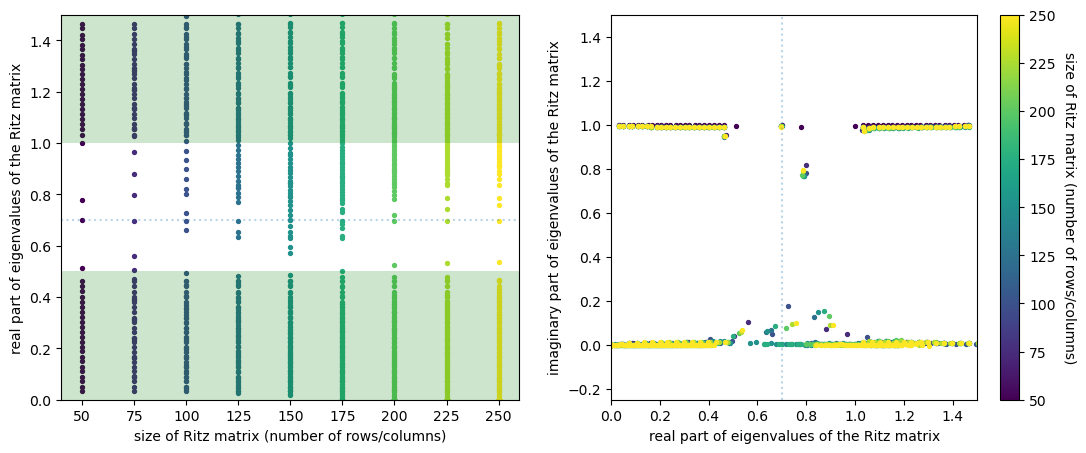
\includegraphics[width=0.9\linewidth, height=6cm]{ptb-mult-dbm}
\caption{The real part of the approximate spectrum for $\tilde{M}+iP$; compare
	with Figure \ref{fig:nodbm}. See that the line at 1.0 on the imaginary
	axis converges to the actual spectrum of the operator, while the
	pollution remains below.}
\label{fig:dbm}
\end{figure}
\clearpage

\begin{remark}
One may also note that there are bands corresponding to the
essential spectrum with imaginary part 1. The reason why dissipative
barriers `replicate' the essential spectrum is an open problem; it has
recently been investigated specifically for Schr\"odinger operators
\cite{stepanenko2022spectral} but in general remains unknown.

Furthermore, additional polluting values can pop up in the complex plane
above the real line, as the operator is no longer self-adjoint!
\end{remark}

As a second example, let us try to replicate some results from Aceto et al.
(2006) \cite{aceto2006numerical}. In this paper, they use an algebraic method
combined with a `shooting technique' to find accurate estimates of specific
eigenvalues for a Sturm-Liouville operator; this algorithm is free from
pollution but works only for a specific class of Sturm-Liouville operators.

\begin{example}\label{ex:aceto} In particular, take the following eigenvalue
	problem on $L^2[0, \infty)$:

$$ \begin{cases} -y'' + (\sin(x) - \frac{40}{1+x^2})y = \lambda y \\ y(0)
\cos(\pi/8) + y'(0) \cos(\pi/8) = 0. \end{cases} $$

This operator has a `band-gap' structure; it has intervals (bands) of essential
spectrum, with eigenvalues dotted in the gaps between bands. In two of
the spectral gaps $J_2 = (-0.34767, 0.59480)$ and $J_3 = (0.91806,
1.2932)$ (denoted in line with the paper and rounded to 5sf) the
algebraic method finds the following eigenvalues:

\begin{figure*}[h!]
\centering \begin{tabular}{c c}
  $J_2$ & $J_3$ \\
  \hline\hline
  0.33594 & 0.94963 \\
  0.53662 & 1.2447 \\
  0.58083 & 1.2919 \\
  0.59150 & \\
\end{tabular}
\end{figure*}

We will attempt to reproduce these eigenvalues using a
Ritz approximation on $[0, \infty)$, with the orthonormal basis
$\{\phi_n\}_{n \in \mathbb{N}}, \phi_n = \exp(-x/2)L_n$, where $L_n$ is
the n'th Laguerre polynomial (see \cite{szego1975orthogonal} for a proof
that this is indeed an orthonormal basis). We will then use a dissipative
barrier to attempt to clear up some spectral pollution.
The result of this approximation is a relative success, 
and is plotted in Figure \ref{fig:aceto-dbm}

Indeed, one benefit of the Galerkin method is that it does not require us to
truncate infinite intervals, which many algebraic methods require; this also
means that we do not have to justify said truncation, which in general may
greatly alter the spectrum!
\end{example}

\begin{figure}[p!]
\centering
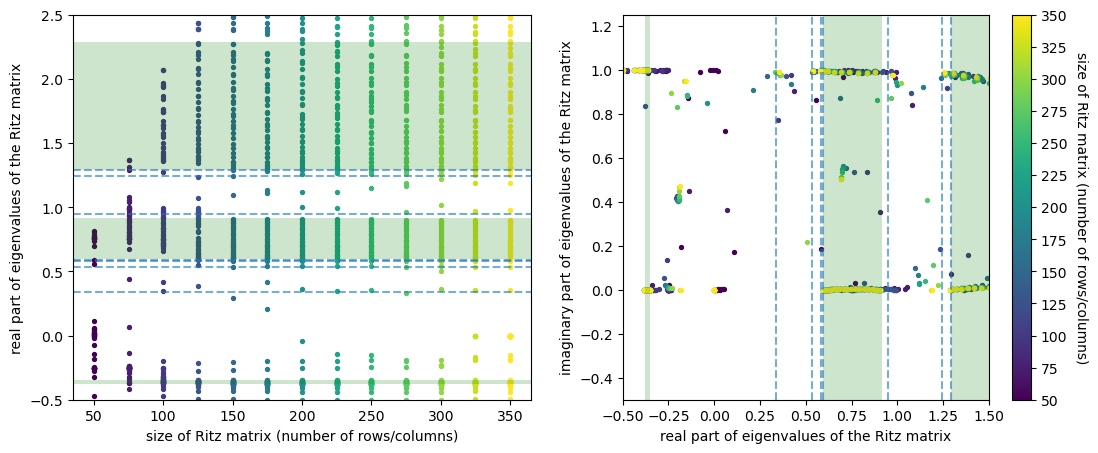
\includegraphics[width=0.9\linewidth, height=6cm]{aceto-dbm}
\caption{The results of a Galerkin approximation with a dissipative
	barrier to the operator of Example \ref{ex:aceto}. The green bands
	represent the essential spectrum of the operator, and the dotted blue
	lines indicate where the algebraic method found eigenvalues in two
	spectral gaps. Note that for larger approximations, the points in the
	spectral gaps with imaginary part 1.0 are close to the algebraic
	method's approximation. The dotted red line will be explained on
  the following page.}
\label{fig:aceto-dbm}
\end{figure}

Interestingly, the non-truncated operator seems to have an additional eigenvalue
not present in the algebraic method, at roughly -0.24. This is denoted
in Figure \ref{fig:aceto-dbm} by a dotted red line. A Galerkin approximation 
of the truncated problem (plotted in Figure \ref{fig:aceto-dbm-bdd})
does not have this eigenvalue, and neither does an approximation of the
same truncated problem in (Marletta, 2010 \cite{marletta2010neumann}) which uses an
oscillation-theory based shooting method \cite{greenberg1997algorithm}. 

\begin{figure}[h!]
\centering
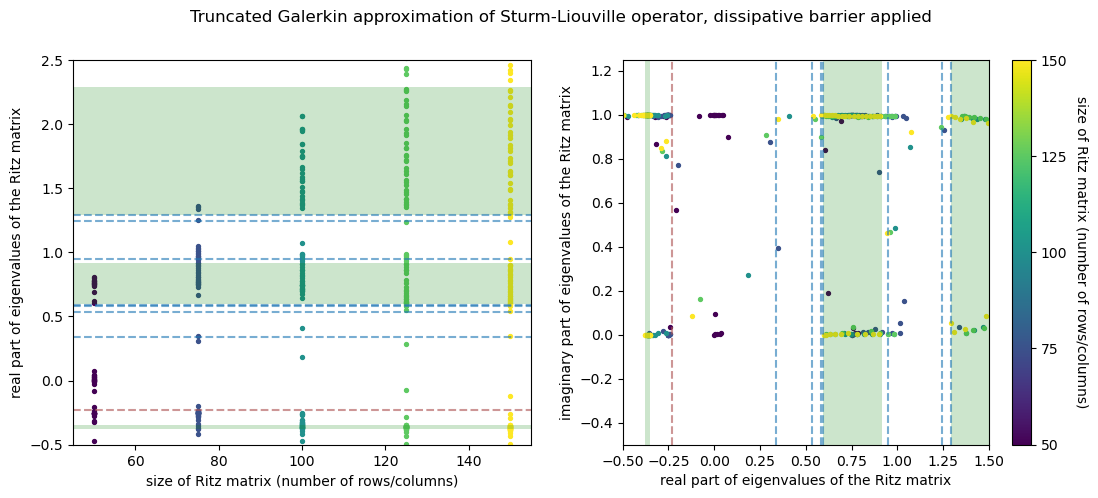
\includegraphics[width=0.9\linewidth, height=6cm]{aceto-dbm-bdd}
\caption{The results of truncating the domain and applying a dissipative
	barrier to the operator of Example \ref{ex:aceto}, with lines and bands
  as above. It has less pollution (as expected; see \cite{aceto2006numerical})
  but is missing the eigenvalue at the red dotted line.}
\label{fig:aceto-dbm-bdd}
\end{figure}

This may be a problem with the dissipative barrier. Indeed, in more generality we can discuss
dissipative barriers of two parameters, $R$ and $\gamma$, where the dissipative barrier is the
quantity $i \gamma \1_{[0, R)}$. We call $R$ the 'length' of the barrier, and $\gamma$ the
'coupling constant' \cite{stepanenko2022spectral}. It is entirely possible that when the barrier
is too long, pollution near the essential spectrum 'jumps up' erroneously.

In figures \ref{fig:dbm-len} and \ref{fig:dbm-coup}, we can see what happens as we vary each of
these parameters to a Galerkin approximation of matrix size 100.
Interestingly, one can see that with a larger coupling constant, eigenvalues
appear to 'jump out' of the essential spectrum and move laterally!

\begin{figure}[p!]
  \centering
  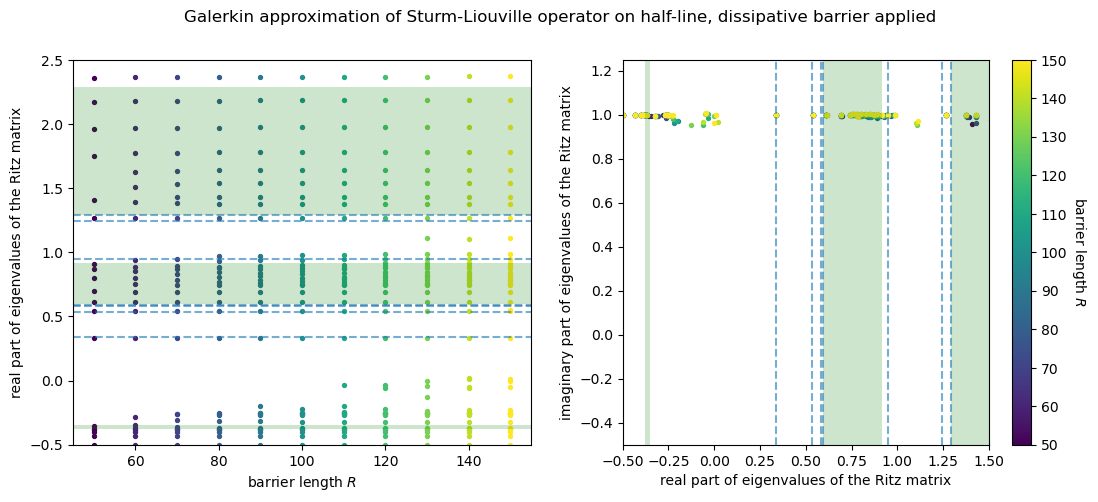
\includegraphics[width=0.9\linewidth, height=6cm]{diss-bar-len}
  \caption{A Galerkin approximation with varying dissipative barrier length,
  with all values of imaginary part less than 0.95 removed. One can see that
  as the barrier length increases, so do the number of eigenvalues pushed up
  by the barrier.}
  \label{fig:dbm-len}
\end{figure}

\begin{figure}[p!]
  \centering
  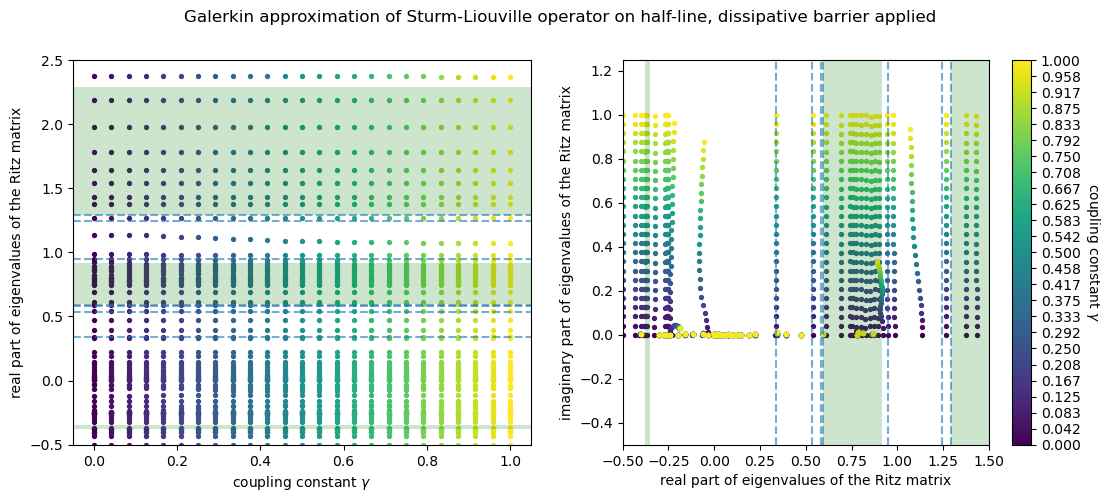
\includegraphics[width=0.9\linewidth, height=6cm]{diss-bar-coup}
  \caption{A Galerkin approximation with varying dissipative coupling constant.
  Note the additional eigenvalues 'jumping out' of the essential spectrum and
  moving around laterally.}
  \label{fig:dbm-coup}
\end{figure}
\clearpage

Finally, this example has some small problems which are worth discussing, as they highlight
a flaw of the Galerkin method in practice. One may notice that when we applied the dissipative barrier,
there is still pollution below the bottom of the essential spectrum (indeed, this pollution
is not there in Figure \ref{aceto-dbm-bdd}). But didn't we say that pollution cannot occur there,
as this is outside of the essential numerical range? It is believed that this is due to inaccuracy
in the numerics that are hard to resolve. 

On one hand, we need to use a large matrix size to
get an accurate estimation of the actual spectrum. On the other, this requires calculating
the integrals of larger and larger basis functions. For the bounded case, this is not a problem,
because we can use quadrature such as Filon quadrature\footnote{'quadrature' meaning 'numerical
integration method'}, which is built to be highly accurate
for oscillatory integrands \cite{chase1969algorithm}. However, in the half-line case, we must
use Gauss-Laguerre quadrature, which is exact for polynomials up to degree $2n-1$ when it is
calculated for $n$ nodes \cite{suli2003introduction}. Thus we either calculate a low number
of nodes and thus suffer inaccuracy from the low-precision quadrature, or calculate a high
number of nodes and suffer inaccuracy in calculating the \emph{nodes themselves}! Devising
Gauss-Laguerre quadrature that remains accurate at high node sizes is a current topic of
research (e.g. \cite{gil2019fast}). The author has seen experimentally that when either of
these inaccuracies occur, they create a 'spread' of eigenvalues around each true eigenvalue,
which is believed to be what is happening here.

Moreover, this shows a flaw of the Ritz and Galerkin methods in general; we need to be able to
accurately calculate inner products of basis functions. This often involves numerical integration
of highly oscillatory functions, which is very difficult to do precisely!
\end{document}
